Для оценки вклада асимметрии, на рис. \ref{ris:assymetric_exp_50}
  приведены результаты двухкристального эксперимента, где в качестве
  кристалла образца и монохроматора использовался кристалл кремния Si(440), но образец был взят таким
  образом, что плоскости (440) располагались под углом $\varphi = 20^o 53^{'}$ к поверхности.

  \begin{figure}[H]
    \centering
    \subfloat[]{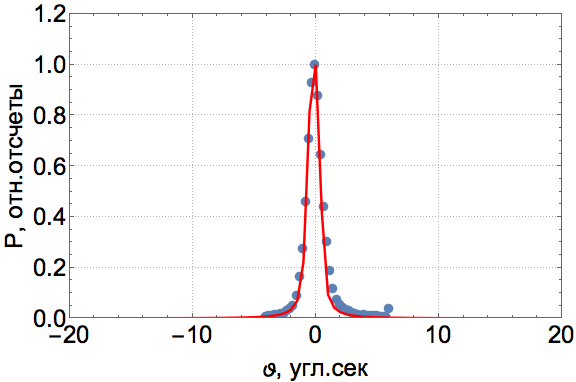
\includegraphics[width=0.4\textwidth]{images/assym-blue-50.png}\label{ris:assymetric_exp_a}}
    \hfill
    \subfloat[]{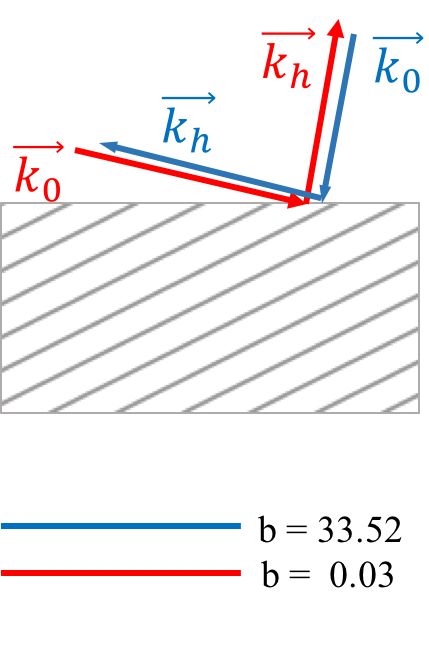
\includegraphics[width=0.15\textwidth]{images/assym_new.png}\label{ris:asym_c}}
    \hfill
    \subfloat[]{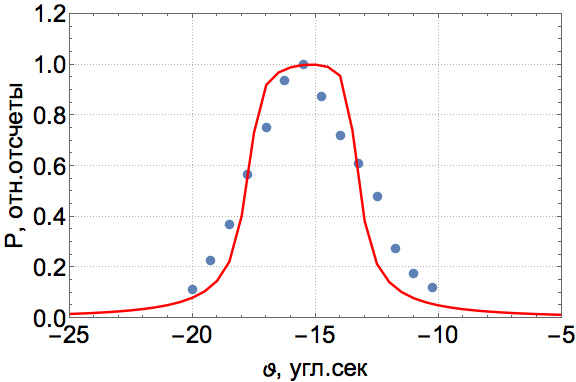
\includegraphics[width=0.4\textwidth]{images/assym-red-50.png}\label{ris:assymetric_exp_b}}

    \caption{Двухкристальная КДО для схемы с установленным кристаллом монохроматором Si(440) и асимметричным образцом Si(440),
    угол разориентации поверхности которого $\varphi = 20^o53^{'}$. Результаты представлены для разных углов падения
    $b = 33.52$, $\varphi$ > 0 (a), $b = 0.03$, $\varphi$ < 0  (с).
     Размер щелевых коллиматоров $S_1 = S_2 = 50$ мкм}
    \label{ris:assymetric_exp_50}
  \end{figure}

Результаты, полученные в ходе эксперимента, находятся в согласии с теорией
В целом, изучение эффекта ассиметрии позволяет сделать вывод, что при использовании резко
асимметричных рефлексов возможно получать двухкристальные КДО, по своей форме
 близкие к собственным кривым образца.

  % Как было показано в разделе \ref{sec:rocking_curve_section}, чтобы получить
  % рентгеновский пучок с очень малой угловой расходимостью необходимо выбирать
  % скользящий угол падения к поверхности кристалла \ref{ris:assymetric_exp_a}.
